% REV01 Sun 27 Jun 2021 14:08:17 WIB
% START Tue 04 May 2021 13:55:16 WIB

\chapter{THE PASSING SHADOW}

The winds and tides rose and fell a certain number of times, the earth
moved round the sun a certain number of times, the ship upon the ocean
made her voyage safely, and brought a baby-Bella home. Then who so blest
and happy as Mrs John Rokesmith, saving and excepting Mr John Rokesmith!

‘Would you not like to be rich NOW, my darling?’

‘How can you ask me such a question, John dear? Am I not rich?’

These were among the first words spoken near the baby Bella as she lay
asleep. She soon proved to be a baby of wonderful intelligence,
evincing the strongest objection to her grandmother’s society, and
being invariably seized with a painful acidity of the stomach when that
dignified lady honoured her with any attention.

It was charming to see Bella contemplating this baby, and finding out
her own dimples in that tiny reflection, as if she were looking in the
glass without personal vanity. Her cherubic father justly remarked
to her husband that the baby seemed to make her younger than before,
reminding him of the days when she had a pet doll and used to talk to it
as she carried it about. The world might have been challenged to produce
another baby who had such a store of pleasant nonsense said and sung
to it, as Bella said and sung to this baby; or who was dressed and
undressed as often in four-and-twenty hours as Bella dressed and
undressed this baby; or who was held behind doors and poked out to stop
its father’s way when he came home, as this baby was; or, in a word, who
did half the number of baby things, through the lively invention of a
gay and proud young mother, that this inexhaustible baby did.

The inexhaustible baby was two or three months old, when Bella began to
notice a cloud upon her husband’s brow. Watching it, she saw a gathering
and deepening anxiety there, which caused her great disquiet. More than
once, she awoke him muttering in his sleep; and, though he muttered
nothing worse than her own name, it was plain to her that his
restlessness originated in some load of care. Therefore, Bella at length
put in her claim to divide this load, and hear her half of it.

‘You know, John dear,’ she said, cheerily reverting to their former
conversation, ‘that I hope I may safely be trusted in great things. And
it surely cannot be a little thing that causes you so much uneasiness.
It’s very considerate of you to try to hide from me that you are
uncomfortable about something, but it’s quite impossible to be done,
John love.’

‘I admit that I am rather uneasy, my own.’

‘Then please to tell me what about, sir.’

But no, he evaded that. ‘Never mind!’ thought Bella, resolutely.
‘John requires me to put perfect faith in him, and he shall not be
disappointed.’

She went up to London one day, to meet him, in order that they might
make some purchases. She found him waiting for her at her journey’s
end, and they walked away together through the streets. He was in gay
spirits, though still harping on that notion of their being rich; and
he said, now let them make believe that yonder fine carriage was theirs,
and that it was waiting to take them home to a fine house they had; what
would Bella, in that case, best like to find in the house? Well! Bella
didn’t know: already having everything she wanted, she couldn’t say.
But, by degrees she was led on to confess that she would like to have
for the inexhaustible baby such a nursery as never was seen. It was
to be ‘a very rainbow for colours’, as she was quite sure baby noticed
colours; and the staircase was to be adorned with the most exquisite
flowers, as she was absolutely certain baby noticed flowers; and there
was to be an aviary somewhere, of the loveliest little birds, as there
was not the smallest doubt in the world that baby noticed birds.
Was there nothing else? No, John dear. The predilections of the
inexhaustible baby being provided for, Bella could think of nothing
else.

They were chatting on in this way, and John had suggested, ‘No jewels
for your own wear, for instance?’ and Bella had replied laughing. O! if
he came to that, yes, there might be a beautiful ivory case of jewels
on her dressing-table; when these pictures were in a moment darkened and
blotted out.

They turned a corner, and met Mr Lightwood.

He stopped as if he were petrified by the sight of Bella’s husband, who
in the same moment had changed colour.

‘Mr Lightwood and I have met before,’ he said.

‘Met before, John?’ Bella repeated in a tone of wonder. ‘Mr Lightwood
told me he had never seen you.’

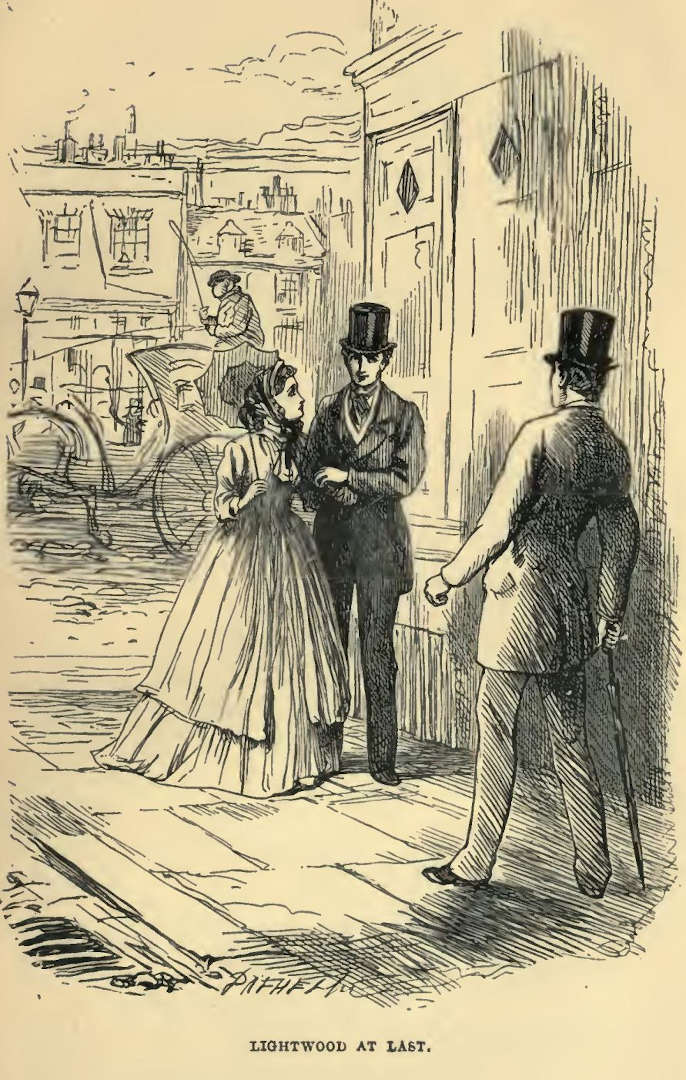
\includegraphics[scale=2.3]{04-12-01}

‘I did not then know that I had,’ said Lightwood, discomposed on her
account. ‘I believed that I had only heard of--Mr Rokesmith.’ With an
emphasis on the name.

‘When Mr Lightwood saw me, my love,’ observed her husband, not avoiding
his eye, but looking at him, ‘my name was Julius Handford.’

Julius Handford! The name that Bella had so often seen in old
newspapers, when she was an inmate of Mr Boffin’s house! Julius
Handford, who had been publicly entreated to appear, and for
intelligence of whom a reward had been publicly offered!

‘I would have avoided mentioning it in your presence,’ said Lightwood to
Bella, delicately; ‘but since your husband mentions it himself, I must
confirm his strange admission. I saw him as Mr Julius Handford, and I
afterwards (unquestionably to his knowledge) took great pains to trace
him out.’

‘Quite true. But it was not my object or my interest,’ said Rokesmith,
quietly, ‘to be traced out.’

Bella looked from the one to the other, in amazement.

‘Mr Lightwood,’ pursued her husband, ‘as chance has brought us face to
face at last--which is not to be wondered at, for the wonder is, that,
in spite of all my pains to the contrary, chance has not confronted
us together sooner--I have only to remind you that you have been at my
house, and to add that I have not changed my residence.’

‘Sir’ returned Lightwood, with a meaning glance towards Bella, ‘my
position is a truly painful one. I hope that no complicity in a very
dark transaction may attach to you, but you cannot fail to know that
your own extraordinary conduct has laid you under suspicion.’

‘I know it has,’ was all the reply.

‘My professional duty,’ said Lightwood hesitating, with another glance
towards Bella, ‘is greatly at variance with my personal inclination; but
I doubt, Mr Handford, or Mr Rokesmith, whether I am justified in taking
leave of you here, with your whole course unexplained.’

Bella caught her husband by the hand.

‘Don’t be alarmed, my darling. Mr Lightwood will find that he is quite
justified in taking leave of me here. At all events,’ added Rokesmith,
‘he will find that I mean to take leave of him here.’

‘I think, sir,’ said Lightwood, ‘you can scarcely deny that when I came
to your house on the occasion to which you have referred, you avoided me
of a set purpose.’

‘Mr Lightwood, I assure you I have no disposition to deny it, or
intention to deny it. I should have continued to avoid you, in pursuance
of the same set purpose, for a short time longer, if we had not met now.
I am going straight home, and shall remain at home to-morrow until noon.
Hereafter, I hope we may be better acquainted. Good-day.’

Lightwood stood irresolute, but Bella’s husband passed him in the
steadiest manner, with Bella on his arm; and they went home without
encountering any further remonstrance or molestation from any one.

When they had dined and were alone, John Rokesmith said to his wife, who
had preserved her cheerfulness: ‘And you don’t ask me, my dear, why I
bore that name?’

‘No, John love. I should dearly like to know, of course;’ (which her
anxious face confirmed;) ‘but I wait until you can tell me of your own
free will. You asked me if I could have perfect faith in you, and I said
yes, and I meant it.’

It did not escape Bella’s notice that he began to look triumphant. She
wanted no strengthening in her firmness; but if she had had need of any,
she would have derived it from his kindling face.

‘You cannot have been prepared, my dearest, for such a discovery as that
this mysterious Mr Handford was identical with your husband?’

‘No, John dear, of course not. But you told me to prepare to be tried,
and I prepared myself.’

He drew her to nestle closer to him, and told her it would soon be over,
and the truth would soon appear. ‘And now,’ he went on, ‘lay stress,
my dear, on these words that I am going to add. I stand in no kind of
peril, and I can by possibility be hurt at no one’s hand.’

‘You are quite, quite sure of that, John dear?’

‘Not a hair of my head! Moreover, I have done no wrong, and have injured
no man. Shall I swear it?’

‘No, John!’ cried Bella, laying her hand upon his lips, with a proud
look. ‘Never to me!’

‘But circumstances,’ he went on ‘--I can, and I will, disperse them in
a moment--have surrounded me with one of the strangest suspicions ever
known. You heard Mr Lightwood speak of a dark transaction?’

‘Yes, John.’

‘You are prepared to hear explicitly what he meant?’

‘Yes, John.’

‘My life, he meant the murder of John Harmon, your allotted husband.’

With a fast palpitating heart, Bella grasped him by the arm. ‘You cannot
be suspected, John?’

‘Dear love, I can be--for I am!’

There was silence between them, as she sat looking in his face, with the
colour quite gone from her own face and lips. ‘How dare they!’ she cried
at length, in a burst of generous indignation. ‘My beloved husband, how
dare they!’

He caught her in his arms as she opened hers, and held her to his heart.
‘Even knowing this, you can trust me, Bella?’

‘I can trust you, John dear, with all my soul. If I could not trust you,
I should fall dead at your feet.’

The kindling triumph in his face was bright indeed, as he looked up and
rapturously exclaimed, what had he done to deserve the blessing of this
dear confiding creature’s heart! Again she put her hand upon his lips,
saying, ‘Hush!’ and then told him, in her own little natural pathetic
way, that if all the world were against him, she would be for him; that
if all the world repudiated him, she would believe him; that if he were
infamous in other eyes, he would be honoured in hers; and that, under
the worst unmerited suspicion, she could devote her life to consoling
him, and imparting her own faith in him to their little child.

A twilight calm of happiness then succeeding to their radiant noon, they
remained at peace, until a strange voice in the room startled them both.
The room being by that time dark, the voice said, ‘Don’t let the lady
be alarmed by my striking a light,’ and immediately a match rattled, and
glimmered in a hand. The hand and the match and the voice were then seen
by John Rokesmith to belong to Mr Inspector, once meditatively active in
this chronicle.

‘I take the liberty,’ said Mr Inspector, in a business-like manner, ‘to
bring myself to the recollection of Mr Julius Handford, who gave me his
name and address down at our place a considerable time ago. Would the
lady object to my lighting the pair of candles on the chimneypiece, to
throw a further light upon the subject? No? Thank you, ma’am. Now, we
look cheerful.’

Mr Inspector, in a dark-blue buttoned-up frock coat and pantaloons,
presented a serviceable, half-pay, Royal Arms kind of appearance, as he
applied his pocket handkerchief to his nose and bowed to the lady.

‘You favoured me, Mr Handford,’ said Mr Inspector, ‘by writing down your
name and address, and I produce the piece of paper on which you wrote
it. Comparing the same with the writing on the fly-leaf of this book on
the table--and a sweet pretty volume it is--I find the writing of the
entry, “Mrs John Rokesmith. From her husband on her birthday”--and very
gratifying to the feelings such memorials are--to correspond exactly.
Can I have a word with you?’

‘Certainly. Here, if you please,’ was the reply.

‘Why,’ retorted Mr Inspector, again using his pocket handkerchief,
‘though there’s nothing for the lady to be at all alarmed at, still,
ladies are apt to take alarm at matters of business--being of that
fragile sex that they’re not accustomed to them when not of a strictly
domestic character--and I do generally make it a rule to propose
retirement from the presence of ladies, before entering upon business
topics. Or perhaps,’ Mr Inspector hinted, ‘if the lady was to step
up-stairs, and take a look at baby now!’

‘Mrs Rokesmith,’--her husband was beginning; when Mr Inspector,
regarding the words as an introduction, said, ‘Happy I am sure, to have
the honour.’ And bowed, with gallantry.

‘Mrs Rokesmith,’ resumed her husband, ‘is satisfied that she can have no
reason for being alarmed, whatever the business is.’

‘Really? Is that so?’ said Mr Inspector. ‘But it’s a sex to live and
learn from, and there’s nothing a lady can’t accomplish when she once
fully gives her mind to it. It’s the case with my own wife. Well, ma’am,
this good gentleman of yours has given rise to a rather large amount
of trouble which might have been avoided if he had come forward and
explained himself. Well you see! He DIDN’T come forward and explain
himself. Consequently, now that we meet, him and me, you’ll say--and say
right--that there’s nothing to be alarmed at, in my proposing to him
TO come forward--or, putting the same meaning in another form, to come
along with me--and explain himself.’

When Mr Inspector put it in that other form, ‘to come along with me,’
there was a relishing roll in his voice, and his eye beamed with an
official lustre.

‘Do you propose to take me into custody?’ inquired John Rokesmith, very
coolly.

‘Why argue?’ returned Mr Inspector in a comfortable sort of
remonstrance; ‘ain’t it enough that I propose that you shall come along
with me?’

‘For what reason?’

‘Lord bless my soul and body!’ returned Mr Inspector, ‘I wonder at it in
a man of your education. Why argue?’

‘What do you charge against me?’

‘I wonder at you before a lady,’ said Mr Inspector, shaking his head
reproachfully: ‘I wonder, brought up as you have been, you haven’t a
more delicate mind! I charge you, then, with being some way concerned
in the Harmon Murder. I don’t say whether before, or in, or after, the
fact. I don’t say whether with having some knowledge of it that hasn’t
come out.’

‘You don’t surprise me. I foresaw your visit this afternoon.’

‘Don’t!’ said Mr Inspector. ‘Why, why argue? It’s my duty to inform you
that whatever you say, will be used against you.’

‘I don’t think it will.’

‘But I tell you it will,’ said Mr Inspector. ‘Now, having received the
caution, do you still say that you foresaw my visit this afternoon?’

‘Yes. And I will say something more, if you will step with me into the
next room.’

With a reassuring kiss on the lips of the frightened Bella, her husband
(to whom Mr Inspector obligingly offered his arm), took up a candle, and
withdrew with that gentleman. They were a full half-hour in conference.
When they returned, Mr Inspector looked considerably astonished.

‘I have invited this worthy officer, my dear,’ said John, ‘to make a
short excursion with me in which you shall be a sharer. He will take
something to eat and drink, I dare say, on your invitation, while you
are getting your bonnet on.’

Mr Inspector declined eating, but assented to the proposal of a glass of
brandy and water. Mixing this cold, and pensively consuming it, he broke
at intervals into such soliloquies as that he never did know such a
move, that he never had been so gravelled, and that what a game was
this to try the sort of stuff a man’s opinion of himself was made
of! Concurrently with these comments, he more than once burst out a
laughing, with the half-enjoying and half-piqued air of a man, who
had given up a good conundrum, after much guessing, and been told the
answer. Bella was so timid of him, that she noted these things in a
half-shrinking, half-perceptive way, and similarly noted that there was
a great change in his manner towards John. That coming-along-with-him
deportment was now lost in long musing looks at John and at herself and
sometimes in slow heavy rubs of his hand across his forehead, as if he
were ironing cut the creases which his deep pondering made there. He had
had some coughing and whistling satellites secretly gravitating towards
him about the premises, but they were now dismissed, and he eyed John as
if he had meant to do him a public service, but had unfortunately been
anticipated. Whether Bella might have noted anything more, if she
had been less afraid of him, she could not determine; but it was all
inexplicable to her, and not the faintest flash of the real state of the
case broke in upon her mind. Mr Inspector’s increased notice of herself
and knowing way of raising his eyebrows when their eyes by any chance
met, as if he put the question ‘Don’t you see?’ augmented her timidity,
and, consequently, her perplexity. For all these reasons, when he
and she and John, at towards nine o’clock of a winter evening went to
London, and began driving from London Bridge, among low-lying water-side
wharves and docks and strange places, Bella was in the state of a
dreamer; perfectly unable to account for her being there, perfectly
unable to forecast what would happen next, or whither she was going, or
why; certain of nothing in the immediate present, but that she confided
in John, and that John seemed somehow to be getting more triumphant. But
what a certainty was that!

They alighted at last at the corner of a court, where there was a
building with a bright lamp and wicket gate. Its orderly appearance was
very unlike that of the surrounding neighbourhood, and was explained by
the inscription POLICE STATION.

‘We are not going in here, John?’ said Bella, clinging to him.

‘Yes, my dear; but of our own accord. We shall come out again as easily,
never fear.’

The whitewashed room was pure white as of old, the methodical
book-keeping was in peaceful progress as of old, and some distant howler
was banging against a cell door as of old. The sanctuary was not a
permanent abiding-place, but a kind of criminal Pickford’s. The lower
passions and vices were regularly ticked off in the books, warehoused in
the cells, carted away as per accompanying invoice, and left little mark
upon it.

Mr Inspector placed two chairs for his visitors, before the fire, and
communed in a low voice with a brother of his order (also of a half-pay,
and Royal Arms aspect), who, judged only by his occupation at the
moment, might have been a writing-master, setting copies. Their
conference done, Mr Inspector returned to the fireplace, and, having
observed that he would step round to the Fellowships and see how matters
stood, went out. He soon came back again, saying, ‘Nothing could be
better, for they’re at supper with Miss Abbey in the bar;’ and then they
all three went out together.

Still, as in a dream, Bella found herself entering a snug old-fashioned
public-house, and found herself smuggled into a little three-cornered
room nearly opposite the bar of that establishment. Mr Inspector
achieved the smuggling of herself and John into this queer room, called
Cosy in an inscription on the door, by entering in the narrow passage
first in order, and suddenly turning round upon them with extended arms,
as if they had been two sheep. The room was lighted for their reception.

‘Now,’ said Mr Inspector to John, turning the gas lower; ‘I’ll mix with
‘em in a casual way, and when I say Identification, perhaps you’ll show
yourself.’

John nodded, and Mr Inspector went alone to the half-door of the bar.
From the dim doorway of Cosy, within which Bella and her husband stood,
they could see a comfortable little party of three persons sitting at
supper in the bar, and could hear everything that was said.

The three persons were Miss Abbey and two male guests. To whom
collectively, Mr Inspector remarked that the weather was getting sharp
for the time of year.

‘It need be sharp to suit your wits, sir,’ said Miss Abbey. ‘What have
you got in hand now?’

‘Thanking you for your compliment: not much, Miss Abbey,’ was Mr
Inspector’s rejoinder.

‘Who have you got in Cosy?’ asked Miss Abbey.

‘Only a gentleman and his wife, Miss.’

‘And who are they? If one may ask it without detriment to your deep
plans in the interests of the honest public?’ said Miss Abbey, proud of
Mr Inspector as an administrative genius.

‘They are strangers in this part of the town, Miss Abbey. They are
waiting till I shall want the gentleman to show himself somewhere, for
half a moment.’

‘While they’re waiting,’ said Miss Abbey, ‘couldn’t you join us?’

Mr Inspector immediately slipped into the bar, and sat down at the side
of the half-door, with his back towards the passage, and directly facing
the two guests. ‘I don’t take my supper till later in the night,’ said
he, ‘and therefore I won’t disturb the compactness of the table. But
I’ll take a glass of flip, if that’s flip in the jug in the fender.’

‘That’s flip,’ replied Miss Abbey, ‘and it’s my making, and if even you
can find out better, I shall be glad to know where.’ Filling him, with
hospitable hands, a steaming tumbler, Miss Abbey replaced the jug by
the fire; the company not having yet arrived at the flip-stage of their
supper, but being as yet skirmishing with strong ale.

‘Ah--h!’ cried Mr Inspector. ‘That’s the smack! There’s not a Detective
in the Force, Miss Abbey, that could find out better stuff than that.’

‘Glad to hear you say so,’ rejoined Miss Abbey. ‘You ought to know, if
anybody does.’

‘Mr Job Potterson,’ Mr Inspector continued, ‘I drink your health. Mr
Jacob Kibble, I drink yours. Hope you have made a prosperous voyage
home, gentlemen both.’

Mr Kibble, an unctuous broad man of few words and many mouthfuls, said,
more briefly than pointedly, raising his ale to his lips: ‘Same to you.’
Mr Job Potterson, a semi-seafaring man of obliging demeanour, said,
‘Thank you, sir.’

‘Lord bless my soul and body!’ cried Mr Inspector. ‘Talk of trades, Miss
Abbey, and the way they set their marks on men’ (a subject which nobody
had approached); ‘who wouldn’t know your brother to be a Steward!
There’s a bright and ready twinkle in his eye, there’s a neatness in his
action, there’s a smartness in his figure, there’s an air of reliability
about him in case you wanted a basin, which points out the steward! And
Mr Kibble; ain’t he Passenger, all over? While there’s that mercantile
cut upon him which would make you happy to give him credit for five
hundred pound, don’t you see the salt sea shining on him too?’

‘YOU do, I dare say,’ returned Miss Abbey, ‘but I don’t. And as for
stewarding, I think it’s time my brother gave that up, and took his
House in hand on his sister’s retiring. The House will go to pieces if
he don’t. I wouldn’t sell it for any money that could be told out, to a
person that I couldn’t depend upon to be a Law to the Porters, as I have
been.’

‘There you’re right, Miss,’ said Mr Inspector. ‘A better kept house is
not known to our men. What do I say? Half so well a kept house is not
known to our men. Show the Force the Six Jolly Fellowship Porters,
and the Force--to a constable--will show you a piece of perfection, Mr
Kibble.’

That gentleman, with a very serious shake of his head, subscribed the
article.

‘And talk of Time slipping by you, as if it was an animal at rustic
sports with its tail soaped,’ said Mr Inspector (again, a subject which
nobody had approached); ‘why, well you may. Well you may. How has it
slipped by us, since the time when Mr Job Potterson here present, Mr
Jacob Kibble here present, and an Officer of the Force here present,
first came together on a matter of Identification!’

Bella’s husband stepped softly to the half-door of the bar, and stood
there.

‘How has Time slipped by us,’ Mr Inspector went on slowly, with his eyes
narrowly observant of the two guests, ‘since we three very men, at an
Inquest in this very house--Mr Kibble? Taken ill, sir?’

Mr Kibble had staggered up, with his lower jaw dropped, catching
Potterson by the shoulder, and pointing to the half-door. He now cried
out: ‘Potterson! Look! Look there!’ Potterson started up, started back,
and exclaimed: ‘Heaven defend us, what’s that!’ Bella’s husband stepped
back to Bella, took her in his arms (for she was terrified by the
unintelligible terror of the two men), and shut the door of the little
room. A hurry of voices succeeded, in which Mr Inspector’s voice was
busiest; it gradually slackened and sank; and Mr Inspector reappeared.
‘Sharp’s the word, sir!’ he said, looking in with a knowing wink. ‘We’ll
get your lady out at once.’ Immediately, Bella and her husband were
under the stars, making their way back, alone, to the vehicle they had
kept in waiting.

All this was most extraordinary, and Bella could make nothing of it but
that John was in the right. How in the right, and how suspected of being
in the wrong, she could not divine. Some vague idea that he had never
really assumed the name of Handford, and that there was a remarkable
likeness between him and that mysterious person, was her nearest
approach to any definite explanation. But John was triumphant; that much
was made apparent; and she could wait for the rest.

When John came home to dinner next day, he said, sitting down on the
sofa by Bella and baby-Bella: ‘My dear, I have a piece of news to tell
you. I have left the China House.’

As he seemed to like having left it, Bella took it for granted that
there was no misfortune in the case.

‘In a word, my love,’ said John, ‘the China House is broken up and
abolished. There is no such thing any more.’

‘Then, are you already in another House, John?’

‘Yes, my darling. I am in another way of business. And I am rather
better off.’

The inexhaustible baby was instantly made to congratulate him, and
to say, with appropriate action on the part of a very limp arm and a
speckled fist: ‘Three cheers, ladies and gemplemorums. Hoo--ray!’

‘I am afraid, my life,’ said John, ‘that you have become very much
attached to this cottage?’

‘Afraid I have, John? Of course I have.’

‘The reason why I said afraid,’ returned John, ‘is, because we must
move.’

‘O John!’

‘Yes, my dear, we must move. We must have our head-quarters in London
now. In short, there’s a dwelling-house rent-free, attached to my new
position, and we must occupy it.’

‘That’s a gain, John.’

‘Yes, my dear, it is undoubtedly a gain.’

He gave her a very blithe look, and a very sly look. Which occasioned
the inexhaustible baby to square at him with the speckled fists, and
demand in a threatening manner what he meant?

‘My love, you said it was a gain, and I said it was a gain. A very
innocent remark, surely.’

‘I won’t,’ said the inexhaustible baby,
‘--allow--you--to--make--game--of--my--venerable--Ma.’ At each division
administering a soft facer with one of the speckled fists.

John having stooped down to receive these punishing visitations, Bella
asked him, would it be necessary to move soon? Why yes, indeed (said
John), he did propose that they should move very soon. Taking the
furniture with them, of course? (said Bella). Why, no (said John), the
fact was, that the house was--in a sort of a kind of a way--furnished
already.

The inexhaustible baby, hearing this, resumed the offensive, and said:
‘But there’s no nursery for me, sir. What do you mean, marble-hearted
parent?’ To which the marble-hearted parent rejoined that there was
a--sort of a kind of a--nursery, and it might be ‘made to do’. ‘Made to
do?’ returned the Inexhaustible, administering more punishment, ‘what do
you take me for?’ And was then turned over on its back in Bella’s lap,
and smothered with kisses.

‘But really, John dear,’ said Bella, flushed in quite a lovely manner
by these exercises, ‘will the new house, just as it stands, do for baby?
That’s the question.’

‘I felt that to be the question,’ he returned, ‘and therefore I arranged
that you should come with me and look at it, to-morrow morning.’
Appointment made, accordingly, for Bella to go up with him to-morrow
morning; John kissed; and Bella delighted.

When they reached London in pursuance of their little plan, they took
coach and drove westward. Not only drove westward, but drove into that
particular westward division, which Bella had seen last when she turned
her face from Mr Boffin’s door. Not only drove into that particular
division, but drove at last into that very street. Not only drove into
that very street, but stopped at last at that very house.

‘John dear!’ cried Bella, looking out of window in a flutter. ‘Do you
see where we are?’

‘Yes, my love. The coachman’s quite right.’

The house-door was opened without any knocking or ringing, and John
promptly helped her out. The servant who stood holding the door, asked
no question of John, neither did he go before them or follow them as
they went straight up-stairs. It was only her husband’s encircling arm,
urging her on, that prevented Bella from stopping at the foot of the
staircase. As they ascended, it was seen to be tastefully ornamented
with most beautiful flowers.

‘O John!’ said Bella, faintly. ‘What does this mean?’

‘Nothing, my darling, nothing. Let us go on.’

Going on a little higher, they came to a charming aviary, in which a
number of tropical birds, more gorgeous in colour than the flowers,
were flying about; and among those birds were gold and silver fish, and
mosses, and water-lilies, and a fountain, and all manner of wonders.

‘O my dear John!’ said Bella. ‘What does this mean?’

‘Nothing, my darling, nothing. Let us go on.’

They went on, until they came to a door. As John put out his hand to
open it, Bella caught his hand.

‘I don’t know what it means, but it’s too much for me. Hold me, John,
love.’

John caught her up in his arm, and lightly dashed into the room with
her.

Behold Mr and Mrs Boffin, beaming! Behold Mrs Boffin clapping her hands
in an ecstacy, running to Bella with tears of joy pouring down her
comely face, and folding her to her breast, with the words: ‘My deary
deary, deary girl, that Noddy and me saw married and couldn’t wish joy
to, or so much as speak to! My deary, deary, deary, wife of John and
mother of his little child! My loving loving, bright bright, Pretty
Pretty! Welcome to your house and home, my deary!’



